%!TEX ROOT=formularioMatematica.tex

\section{Geometria analitica nello spazio}
La geometria analitica non erelativa esclusivamente a piani bidimensionali. Di seguito verrano 
proposte le formule e spiegazioni di quella in tre dimensioni.
\subsection{Vettori}
Molto spesso si utilizzerà il concetto di \emph{vettore}.Un vettore può essere rappresentato in 
molti modi, tra cui:
\begin{equation*}
  \vec{v} = 
  \begin{bmatrix}[1]
    a\\b\\\vdots
  \end{bmatrix} = 
  (a, b, \dots)
\end{equation*}
Un vettore è composto di un numero definito di \emph{componenti}, solitamente una per ciascuna
dimensione in cui si lavora. Quindi è decisamente più comune trovare vettori \emph{bidimensionali}
che non con un numero maggiore di componenti.
\begin{center}
  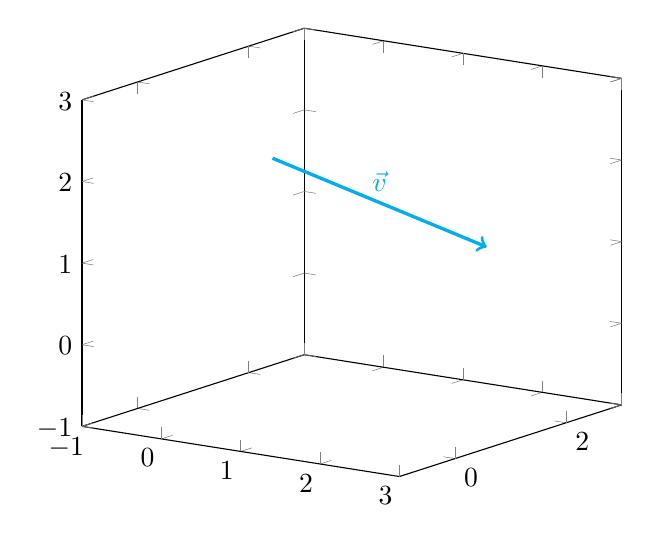
\begin{tikzpicture}
    \begin{axis}[xmin=-1,ymin=-1,zmin=-1,xmax=3,ymax=3,zmax=3,view={35}{15}]
      \addplot3[very thick,->,cyan] coordinates {(0,1,2) (2,2,1)}
        node[pos=0.5,above]{$\vec{v}$};
    \end{axis}
  \end{tikzpicture}
\end{center}
In questa immagine è possibile vedere un vettore $\mathcolor{cyan}{\vec{v}}(x,y,z)$ e le sue 
componenti.\\[\baselineskip]
D'ora in poi sarà dato per scontato che i vettori siano tri-dimensionali.

\subsubsection{Operazioni tra vettori}
Le operazioni come addizione e sottrazione funzionano molto semplicemente sommando algebricamente
le componenti tra di loro:
\begin{equation*}
  \mathcolor{red}{\vec{v_1}\left(x_1, y_1, z_1\right)} \pm 
  \mathcolor{blue}{\vec{v_2}\left(x_2, y_2, z_1\right)} = 
  \mathcolor{purple}{\vec{v}}\left(\mathcolor{red}{x_1}\pm \mathcolor{blue}{x_2}, 
  \mathcolor{red}{y_1}\pm \mathcolor{blue}{y_2},
  \mathcolor{red}{z_1}\pm \mathcolor{blue}{z_2}\right)
\end{equation*}

La moltiplicazione tra vettori può avere come risultato o un \emph{vettore} o uno \emph{scalare}.

\subsubsection{Prodotto scalare}
\begin{equation*}
  \mathcolor{red}{\vec{v_1}} \cdot \mathcolor{blue}{\vec{v_2}} = 
  \mathcolor{red}{x_1}\mathcolor{blue}{x_2} + \mathcolor{red}{y_1}\mathcolor{blue}{y_2}+
  \mathcolor{red}{z_1}\mathcolor{blue}{z_2}
\end{equation*}
Come si può notare il prodotto scalare tra due vettori torna uno scalare (ovvero un numero).
È molto comune trovare questa definizione di prodotto scalare:
\begin{equation*}
  \mathcolor{red}{\vec{v_1}} \cdot \mathcolor{blue}{\vec{v_2}} =
  \norm{\mathcolor{red}{\vec{v_1}}}\cdot\norm{\mathcolor{blue}{\vec{v_2}}}\cos\theta
\end{equation*}
$\norm{\vec{v}}$ è il modulo del vettore $\vec{v}$, ovvero la sua lunghezza. $\theta$ è l'angolo
formato dai due vettori. Si noti che
\begin{equation*}
  \norm{\vec{v}} = \sqrt{x^2+y^2+z^2} 
\end{equation*}

\subsubsection{Prodotto vettoriale}\label{subsec:vettori:prodottoVettoriale}
\begin{equation*}
  \mathcolor{red}{\vec{v_1}} \times \mathcolor{blue}{\vec{v_2}} =
  n\norm{\mathcolor{red}{\vec{v_1}}}\cdot\norm{\mathcolor{blue}{\vec{v_2}}}\sin\theta
\end{equation*}
$\norm{\vec{v}}$ è il modulo del vettore $\vec{v}$, ovvero la sua lunghezza. $\theta$ è l'angolo
formato dai due vettori. $n$ è la \emph{normale} del piano su cui stanno i vettori. 
Una \emph{normale} è un vettore perpendicolare ad un oggetto dato.\\
Per scoprire la direzione del nuovo vettore si può usare la così detta ``regola della mano''. Essa 
dice:
\begin{enumerate}
  \item Usare il pollice della mano destra in direzione e verso del \textbf{primo} vettore
  \item Usare l'indice o le altre dite in direzione e verso del \textbf{secondo} vettore
  \item Il nuovo vettore avrà la direzione che attraversa il palmo perpendicolarmente e il vers
    o uscente dalla mano.
\end{enumerate}

\subsubsection{Angolo tra vettori}
\begin{center}
  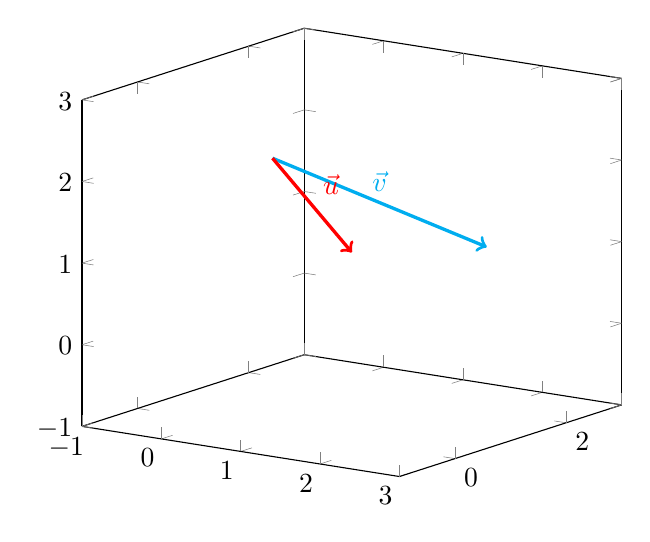
\begin{tikzpicture}
    \begin{axis}[xmin=-1,ymin=-1,zmin=-1,xmax=3,ymax=3,zmax=3,view={35}{15}]
      \addplot3[very thick,cyan,->] coordinates {(0,1,2) (2,2,1)}
        node[pos=0.5,above]{$\vec{v}$};
      \addplot3[very thick,red,->] coordinates {(0,1,2) (1,1,1)}
        node[pos=0.5,above right]{$\vec{u}$};
    \end{axis}
  \end{tikzpicture}
\end{center}
Partendo dalla definizione precedente abbiamo che
\begin{equation*}
  \vec{v}\cdot\vec{v}=(x_v x_u,y_u y_v,z_u z_v)=\norm{v}\norm{u}\cos\theta
\end{equation*}
Invertendo si ottiene semplicemente
\begin{equation*}
  \cos\theta=\frac{\vec{v}\cdot\vec{v}}{\norm{v}\norm{u}}=
  \frac{x_v x_u+y_v y_u+z_v z_u}{\sqrt{x_v^2+y_v^2+z_v^2}\sqrt{x_u^2+y_u^2+z_u^2}}
\end{equation*}

\subsection{Piani}
Come definire l'equazione del piano nello spazio? Ci sono due modi per esprimerlo: in forma 
parametrica o geometrica/analitica.
\subsubsection{Forma parametrica}
L'idea è di prendere un punto $P(x,y,z)$ nello spazio e un punto $P_0(x_0,y_0,z_0)$. Si prendono 
inoltre due vettori $\vec{u}$ e $\vec{v}$ a partire da $P_0$ in modo che la loro somma sia 
$\overline{PP_0}$.
\begin{center}
  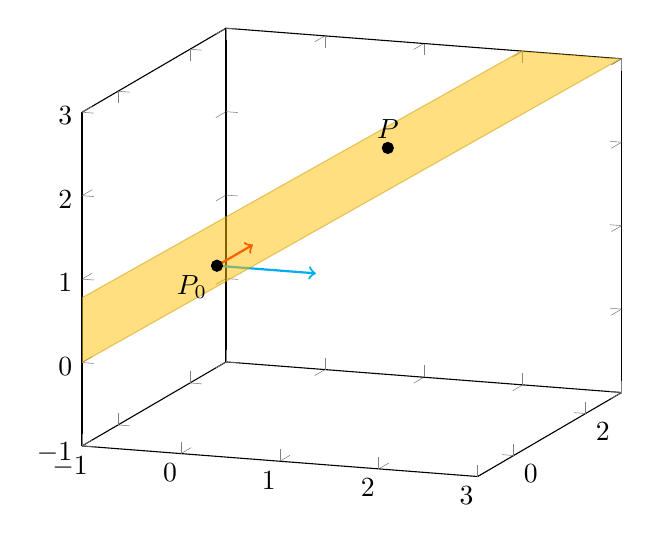
\begin{tikzpicture}
    \begin{axis}[xmin=-1,ymin=-1,zmin=-1,xmax=3,ymax=3,zmax=3,view={20}{15}]
      \coordinate (P0) at (0,0,1);
      \coordinate (P) at (1,2,2);
      \addplot3[only marks] coordinates {(0,0,1) (1,2,2)};
      \addplot3[thick, ->,cyan] coordinates {(0,0,1) (1,0,1)};
      \addplot3[thick, ->,red] coordinates {(0,0,1) (0,1,1)};
      \addplot3[surf,opacity=0.5] coordinates 
        {
          (-1,-1,0) (3,4,3)

          (-2,1,0) (2,4,3)
      };

      \node[below left] at (axis cs:0,0,1) {$P_0$};
      \node[above] at (axis cs:1,2,2) {$P$};
    \end{axis}
  \end{tikzpicture}
\end{center}
$\vec{u}$ e $\vec{v}$ sono linearmente dipendenti dato che la loro somma deve essere 
$\overline{P_0P}$. Se i due vettori giaciono su di un piano $\pi$, allora anche il vettore somma
lo farà. Si ha quindi che, per due costanti $\lambda$ e $\mu$
\begin{equation*}
  \vec{OP}=\vec{OP_0}+\vec{P_0P} = \vec{OP_0}+\lambda\vec{v}+\mu\vec{u}
\end{equation*}
Per la proprietà distributiva si può scrivere
\begin{equation*}
  (x,y,z)=(x_0,y_0,z_0)+(\lambda v_x,\lambda v_y,\lambda v_z)+(\mu u_x,\mu u_y,\mu u_z)
\end{equation*}
E si ottiene quindi un sistema
\begin{equation*}
  \begin{cases}
    x &= x_0+\lambda v_x +\mu u_x\\
    y &= y_0+\lambda v_y +\mu u_y\\
    z &= z_0+\lambda v_z +\mu u_z\\
  \end{cases}
\end{equation*}

\subsubsection{Geometrica}
Si prendono due punti $Q(a,b,c)$ e $P(x,y,z)$ in modo che si ha un angolo retto tra i segmenti
$\overline{OQ}$ e $\overline{QP}$.
\begin{center}
  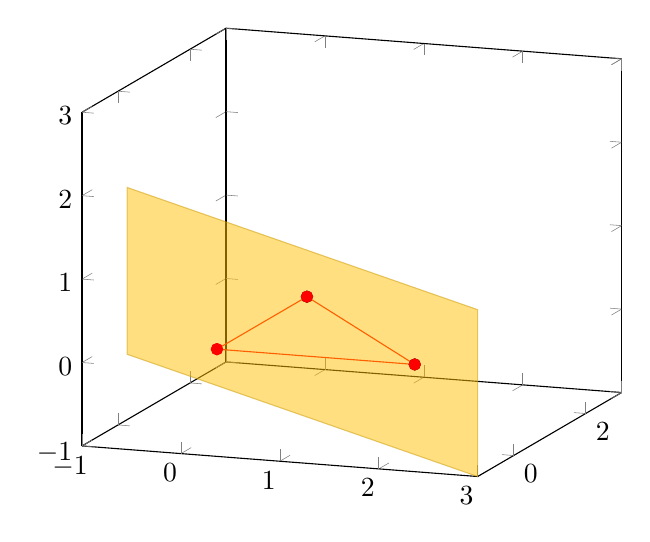
\begin{tikzpicture}
    \begin{axis}[xmin=-1,ymin=-1,zmin=-1,xmax=3,ymax=3,zmax=3,view={20}{15}]
      \addplot3[only marks] coordinates {(2,0,0) (0,2.5,0)};
      \addplot3[mark=*,red] coordinates {(0,0,0) (2,0,0) (0,2.5,0) (0,0,0)};
      \addplot3[surf,opacity=0.5] coordinates {
          (3,-1,-1) (3,-1,1)

          (-2,3,-1) (-2,3,1)
        };
    \end{axis}
  \end{tikzpicture}
\end{center}
Quindi abbiamo
\begin{align*}
  x^2+y^2+z^2&=a^2+b^2+c^2+(x-a)^2+(y-b)^2+(z-c)^2\\
  0&=ax+by+cz-a^2-b^2-c^2\\
  0&=ax+by+cz+d
\end{align*}
